\section{Differential Equations}
    \begin{frame}{Solving Differential Equations}
	    Differentiation is linear!
	    
	    $$\frac{d(c_1x(t) + c_2y(t))}{dt} = c_1\frac{dx(t)}{dt} + c_2\frac{dy(t)}{dt}$$
	\end{frame}
	
	\begin{frame}{Solving systems of differential equations}
	    Write the system in the following form:

        $$\frac{dx(t)}{dt} = Ax(t)$$
        
        Find the eigenvalues/eigenvectors of $A$ and transform the system into the eigenbasis. If $A$ has distinct eigenvalues, the general solution is:
        
        $$x(t) = c_1e^{\lambda_1{t}}\vec{v_1} + c_2e^{\lambda_2{t}}\vec{v_2}$$
        
        Then, change back to the standard basis.
	\end{frame}
	
	\begin{frame}{Example: second-order differential equations}
	    Solve the following differential equation:

        $$\ddot{x} - \dot{x} - 2x = 0$$
        
        $$x(0) = 2, \dot{x}(0) = 1$$
	\end{frame}
	
	\begin{frame}{Example: second-order differential equations}
	    $\ddot{x} - \dot{x} - 2x = 0$, $x(0) = 2, \dot{x}(0) = 1$
	    
	    Solution:
	    
	    Write in matrix form and find eigenvectors:
	    $$\mat{\dot{x};\ddot{x}} = \mat{0 1; 2 1}\mat{x;\dot{x}}$$
	    
	    $$\lambda_1 = 2, v_1 = \mat{1;2}, \lambda_2 = -1, v_2 = \mat{-1;1}$$
	    
	    Use general form to solve:
	    
	    $$\mat{x;\dot{x}} = c_1e^{2t}v_1 + c_2e^{-t}v_2$$
	\end{frame}
	
	\begin{frame}{Example: second-order differential equations}
	    $\ddot{x} - \dot{x} - 2x = 0$, $x(0) = 2, \dot{x}(0) = 1$
	    
	    Solution:
	    
	    Now plug in initial conditions:
	    $$\mat{2;1} = \mat{x(0); \dot{x}(0)} = c_1v_1 + c_2v_2 = \mat{c_1-c_2;2c_1+c_2}$$
	    
	    Solving, we get $c_1 = 1, c_2 = -1$
	    
	    so $x(t) = e^{2t} + e^{-t}$
	\end{frame}
	
	\begin{frame}{Example: second-order differential equations}
	    $\ddot{x} - \dot{x} - 2x = 0$, $x(0) = 2, \dot{x}(0) = 1$
	    
	    Solution:
	    
	    Sanity check: compute derivatives and check that the original system is satisfied
	    
	    $x(t) = e^{2t} + e^{-t}, \dot{x}(t) = 2e^{2t} - e^{-t}, \ddot{x}(t) = 4e^{2t} + e^{-t}$
	    
	    $\implies \ddot{x} - \dot{x} - 2x = 0, x(0) = 2, \dot{x}(0) = 1$
	\end{frame}
	
	\begin{frame}{Example: second-order differential equations}
	    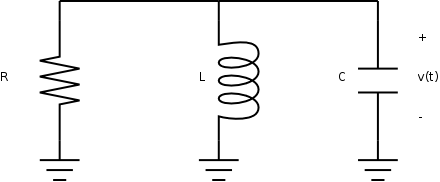
\includegraphics[width=0.6\textwidth]{./images/second-order-1.png}
	    
	    Given $x(t) = \mat{v(t);i_L(t)}$
	    
	    find matrix $A$ such that $\frac{dx}{dt} = Ax$
	\end{frame}
	
	\begin{frame}{Example: second-order differential equations}
    	\begin{columns}[onlytextwidth,T]
        	\column{\dimexpr\linewidth-40mm-5mm}
        	Direct all currents into ground.
	        
	        $$i_R + i_L + i_C = 0$$
	        
	        $$\frac{V}{R} + i_L = -C\frac{dV}{dt}$$
	        
	        $$-\frac{1}{CR}V + -\frac{1}{C}i_L = \frac{dV}{dt}$$
	        
	        Also $L\frac{di_L}{dt} = V \implies A = \mat{-\frac{1}{RC} -\frac{1}{C}; \frac{1}{L} 0}$
	        
	        \column{40mm}
	        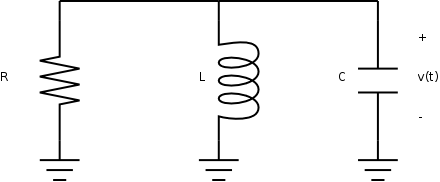
\includegraphics[width=40mm]{./images/second-order-1.png}
        \end{columns}
	\end{frame}
	
	\begin{frame}{Example: second-order differential equations}
	    \begin{columns}[onlytextwidth,T]
        	\column{\dimexpr\linewidth-40mm-5mm}
        	    At $t < 0$, the circuit is at steady state. At $t \geq 0$, the voltage source is set to 0. Find a differential equation for $i_L$ for $t \geq 0$.
        	
        	\column{40mm}
        	    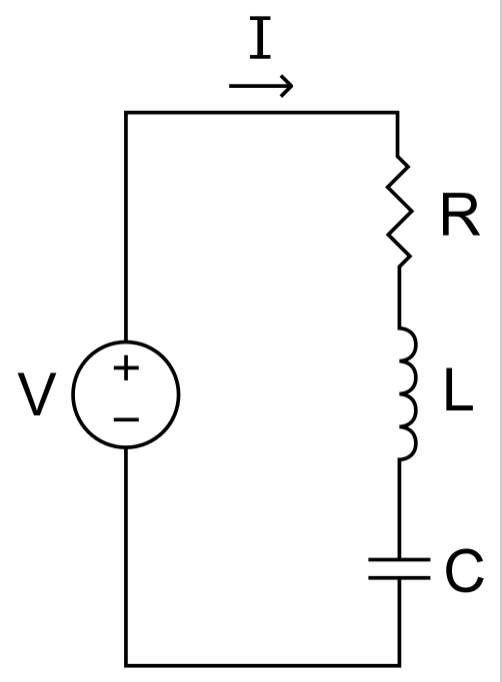
\includegraphics[width=40mm]{./images/second-order-2.png}
    	\end{columns}
	\end{frame}
	
	\begin{frame}{Example: second-order differential equations}
	    \begin{columns}[onlytextwidth,T]
        	\column{\dimexpr\linewidth-40mm-5mm}
        	    Solution: use KCL/KVL to get
        	    
        	    $$i_R = i_L = i_C, V_C + V_R + V_L = 0$$
        	    
        	    $$\frac{V_R}{R} = i_L = C\frac{dV_C}{dt}, \frac{1}{C}i_L + R\frac{di_L}{dt} + L\frac{d^2i_L}{dt} = 0$$
        	    
        	    $$\mat{\frac{di_L}{dt}; \frac{d^2i_L}{dt}} = \mat{0 1; -\frac{1}{LC} -\frac{R}{L}}\mat{i_L;\frac{di_L}{dt}}$$
        	    
        	\column{40mm}
        	    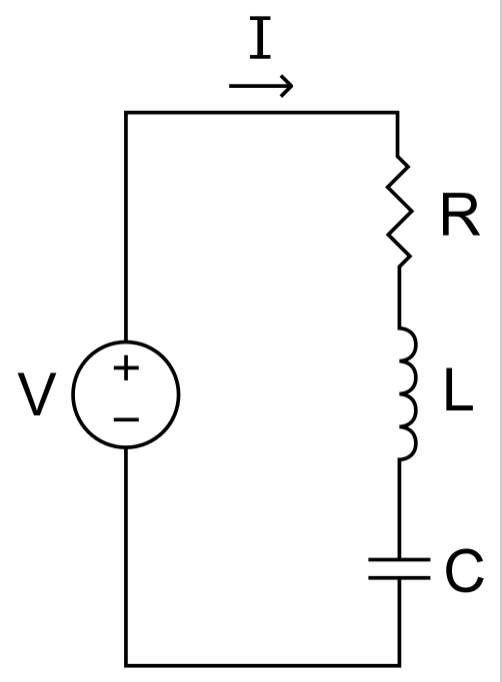
\includegraphics[width=40mm]{./images/second-order-2.png}
    	\end{columns}
	\end{frame}
	
	\begin{frame}{Example: second-order differential equations}
	    \begin{columns}[onlytextwidth,T]
        	\column{\dimexpr\linewidth-40mm-5mm}
        	    If $R = 0$, $L = C = 1$, solve the differential equation:
        	    
        	    Initial conditions: $i_L(0) = 0$, $\frac{di_L}{dt}(0) = -V_c = -V$
        	    
        	    Differential equation: $\mat{\frac{di_L}{dt}; \frac{d^2i_L}{dt}} = \mat{0 1; -\frac{1}{LC} -\frac{R}{L}}\mat{i_L;\frac{di_L}{dt}}$
        	    
        	    $$\lambda_1 = i, v_1 = \mat{i;-1}$$
        	    
        	    $$\lambda_2 = -i, v_2 = \mat{i;1}$$
        	    
        	\column{40mm}
        	    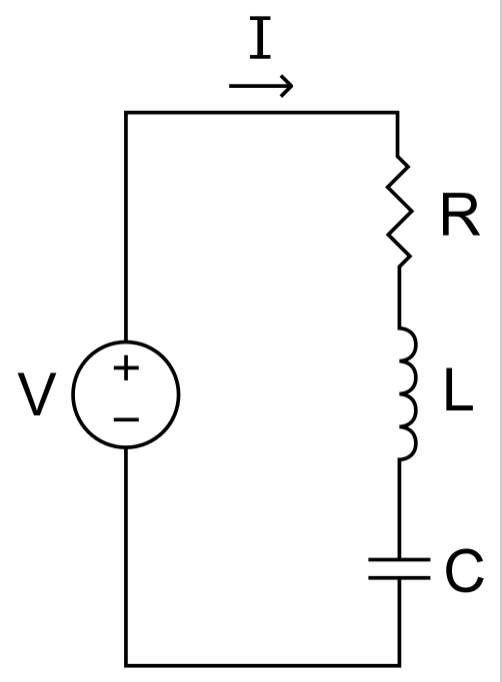
\includegraphics[width=40mm]{./images/second-order-2.png}
    	\end{columns}
	\end{frame}
	
	\begin{frame}{Example: second-order differential equations}
	    \begin{columns}[onlytextwidth,T]
        	\column{\dimexpr\linewidth-40mm-5mm}
        	    $$\mat{i_L;\frac{di_L}{dt}} = c_1e^{it}v_1 + c_2e^{-it}v_2$$
        	    
        	    $$ic_1 + ic_2 = 0, -c_1 + c_2 = -V$$
        	    
        	    $$\implies c_1 = \frac{V}{2}, c_2 = -\frac{V}{2}$$
        	    
        	    so
        	    
        	    $$i_L = \frac{V}{2}ie^{it} - \frac{V}{2}e^{-it}$$
        	    
        	\column{40mm}
        	    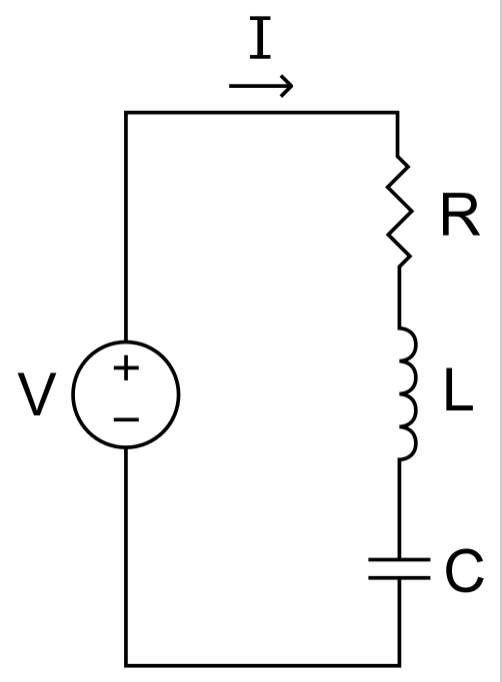
\includegraphics[width=40mm]{./images/second-order-2.png}
    	\end{columns}
	\end{frame}
	
	\begin{frame}{Example: 2 coupled diff eqs}
	    Consider a system of 2 coupled harmonic oscillators, described by

        $$m_i\ddot{x}_i = -(k + \kappa)x_i + \kappa{}x_j$$
        
        \begin{center}
            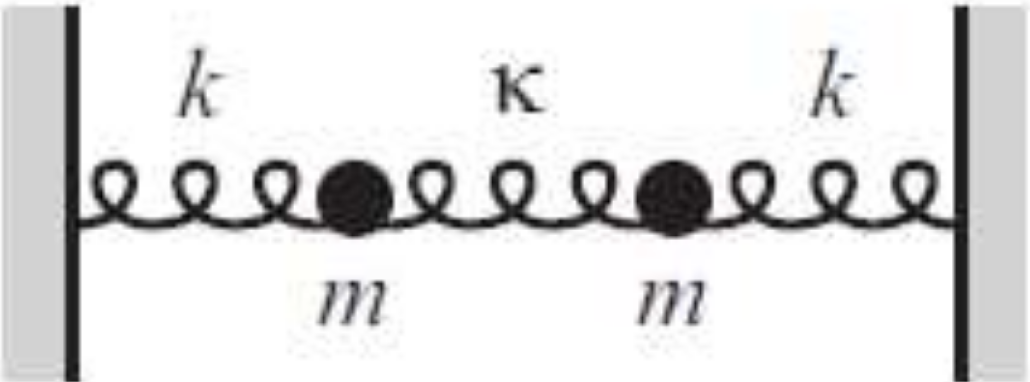
\includegraphics[width=0.5\textwidth]{./images/coupled-eq-1.png}
        \end{center}
	\end{frame}
	
	\begin{frame}{Example: Coupled Oscillator}
	    Write this system in matrix form
        
        $$m_i\ddot{x}_i = -(k + \kappa)x_i + \kappa{}x_j$$
	\end{frame}
	
	\begin{frame}{Example: Coupled Oscillator}
	    Write this system in matrix form
        
        $$m_i\ddot{x}_i = -(k + \kappa)x_i + \kappa{}x_j$$
        
        \begin{center}
         \scalebox{2}{$\ddot{\vec{x}} = \mat{-\frac{k+\kappa}{m} \frac{\kappa}{m}; \frac{\kappa}{m} -\frac{k+\kappa}{m}}\vec{x}$}
        \end{center}
	\end{frame}
	
	\begin{frame}{Example: Coupled Oscillator}
	    Now, diagonalize the system

	    \begin{center}
         \scalebox{2}{$\mat{-\frac{k+\kappa}{m} \frac{\kappa}{m}; \frac{\kappa}{m} -\frac{k+\kappa}{m}} = PDP^{'}$}
        \end{center}
        
        P = ?
        
        D = ?
	\end{frame}
	
	\begin{frame}{Example: Coupled Oscillator}
	    Now, diagonalize the system

	    \begin{center}
         \scalebox{2}{$\mat{-\frac{k+\kappa}{m} \frac{\kappa}{m}; \frac{\kappa}{m} -\frac{k+\kappa}{m}} = PDP^{'}$}
        \end{center}
        
        $$P = \mat{1 1; 1 -1}$$
        
        $$D = \mat{k 0; 0 2\kappa+k}$$
	\end{frame}
	
	\begin{frame}{Example: Coupled Oscillator}
	    $$P = \mat{1 1; 1 -1}$$
        
        $$D = \mat{k 0; 0 2\kappa+k}$$
        
        Since our original matrix was linearly taking a SECOND derivative in time, with only real eigenvalues, we expect solutions to be in the form of real sinusoids, optionally phaseshifted.

        $$x(t) = A_s\mat{1;1}\cos(\sqrt{\frac{k}{m}}t + \phi_s) + A_f\mat{1;-1}\sin(\sqrt{\frac{k + 2\kappa}{m}}t + \phi_f)$$
	\end{frame}
	
